% This example poster is from Scientific Career Resources
%
% Author:
% Chris Rackauckas <contact@chrisrackauckas.com>
% http://www.chrisrackauckas.com

\documentclass[papersize={48in,36in},dvipsnames,fontmag=.60]{umbcposter}

\usepackage{times}
\usepackage{url}
\usepackage{amsmath}
\definecolor{headerGrey}{RGB}{222,222,224}
\definecolor{dBlue}{RGB}{2,45,96}
\definecolor{lBlue}{RGB}{2,66,114}

% Change the font to Computer Modern Sans Serif
% The default is Times New Roman
\renewcommand{\rmdefault}{cmss}

\begin{document}

\newcommand{\mytitle}{
    \tikz \node[
            fill=white,
            draw=dBlue,                   % draw box border
            rounded corners=2ex,
            opacity=0.75,                % background opacity
            text opacity=.9,             % text opacity
            inner sep=0.15\headheight,  % padding around the text
        ] at (0,0) {
            \begin{tabular}{c}
                \Huge
                    Independent Mean/Variance Regulation in the
                    Self-Enhanced Degradation Motif \\
                \huge Chris Rackauckas, Likun Zheng, Julian Sosnik, Tom Schilling, Qing Nie
            \end{tabular}
    };    % don't forget the semicolon here!
}


\posterinit{
	%grid,
	columns = {3},
  	background command = {
     		\path (current page.center) node {
         		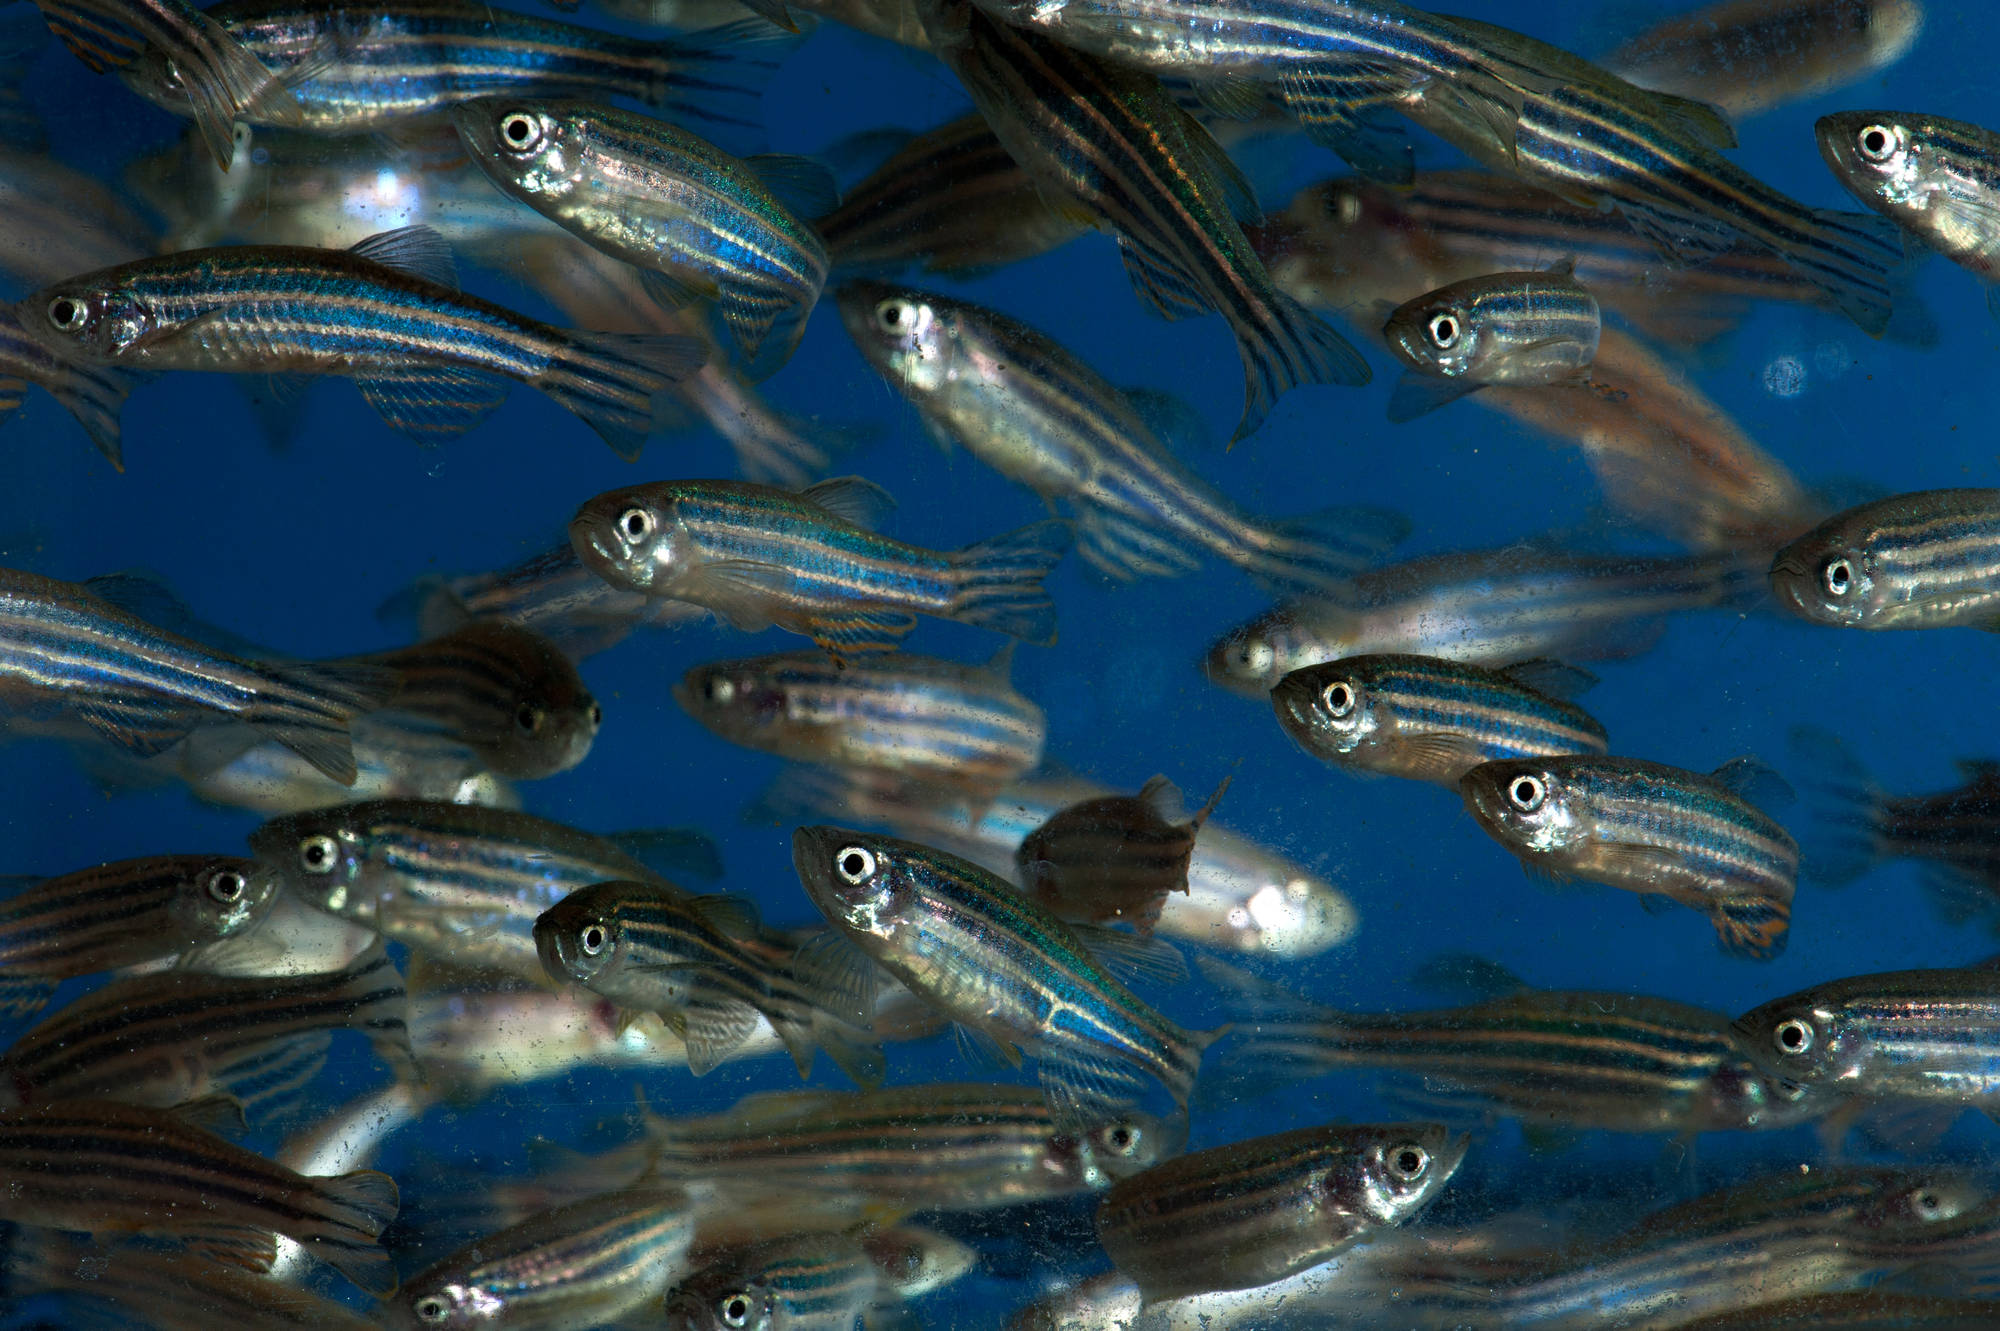
\includegraphics[width=\paperwidth,height=\paperheight]{figures/zebrafish.jpg}};
   	},
	title = {\mytitle},
	left logo = {
\includegraphics[height=.33\headheight]{../uciLogos/AyalaLogos/UCI_FJA_SBS_LOGO_HOR_FIN_DNA_RGB_R.jpg}},
	right logo = {
\includegraphics[height=.75\headheight]{../uciLogos/CCBS/CCBS_GlowBallsWBG.pdf}},
	box/border style= {draw = dBlue, line width = 1pt},
	box/header style = {top color = dBlue, bottom color = dBlue, middle color = lBlue, fill opacity = .9},
	box/header font color = {headerGrey},
	box/header font = {\large\rm},
	box/body style = {fill = white, fill opacity=.85},
	head height = {0.15\textheight},
	box/all rounded
}

\boxit{col = 0, at top, name=problem}{The Zebrafish Hindbrain}{
	\begin{itemize}
\item The hindbrain is segmented due to spatial patterning of the Hox genes.
\item This portion of the brain, known as the ``hindbrain`` or the ``brainstem``, collectively regulates vital bodily processes
such as breathing, swallowing, blood circulation, and muscle tone.
\item Signals produced by mesoderm lying posterior to the hindbrain include RA, and FGF, which with the help of the HOX genes help divide
the hindbrain into rhombomeres. 
\item We wish to understand how noise contributes and is regulated within this spatial patterning network.
\end{itemize}

\begin{center}
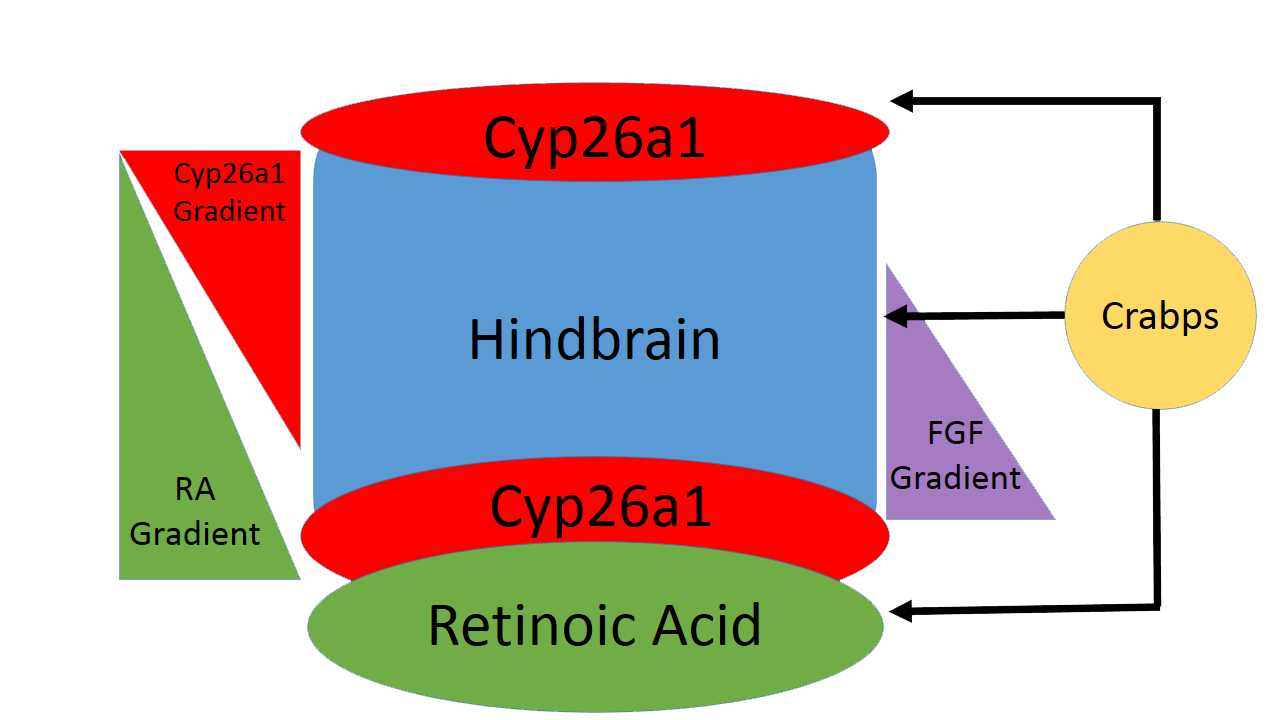
\includegraphics[scale=0.25]{figures/RAcartoons}
\par\end{center}
	\vspace{10pt}
}

\boxit{col = 0, below of = problem, name=box2}{The Interaction Network}{
	\begin{tabular}{c c}
\hspace{-15pt}
{\parbox{.45\textwidth}{\begin{itemize}
\item Cells unleash RA from nutrients in the yolk. 
\item Cyp26a1 is an intracellular (non-diffusive) molecule which degrades RA.
\item Receptor-bound RA (RA-R) upregulates the production of Cyp26a1, creating a self-enhanced degradation loop.
\item Cellular retonoic acid binding proteins (Crabps) can both help deliver RA to its receptors as well as deliver it to Cyp26s for degradation. One of these, Crabp2a, is also induced by RA and can increase self-enhanced degradation.
\end{itemize}}}
&
\raisebox{-.45\totalheight}{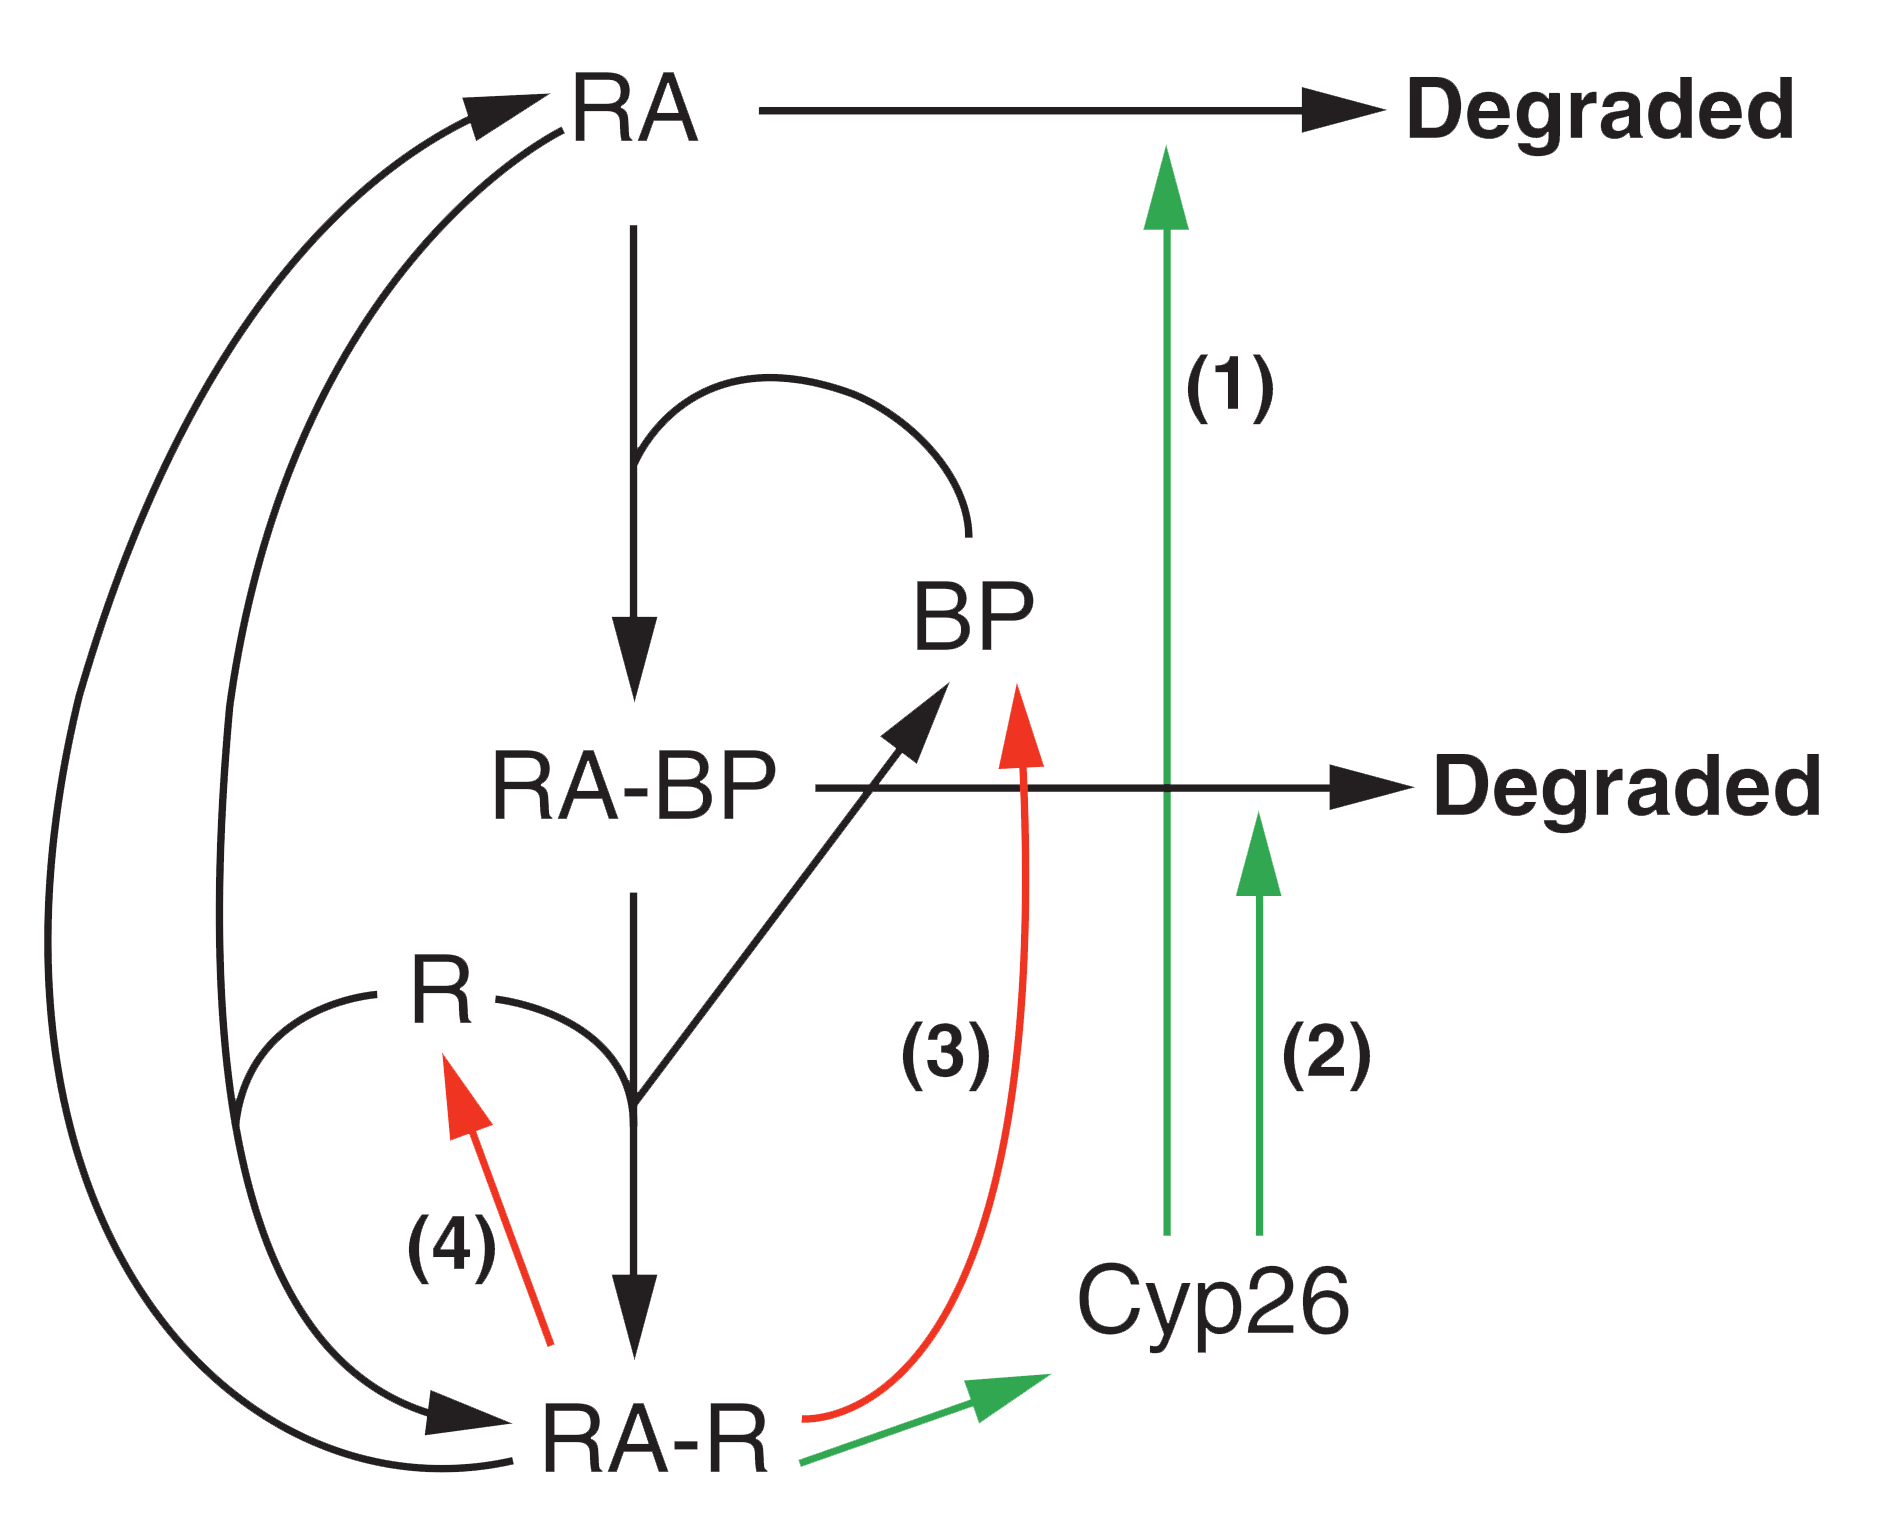
\includegraphics[scale=0.093]{figures/RANetwork.PNG}}
\end{tabular}

	\vspace{5.3pt}
}

\boxit{at top, col = 1, name=box3}{Phenomenological Model}{
	We wish to model the effects of the cellular retinoic acid binding proteins
(crabps) and Cyp26a1 on the noise of the RA gradiant in zebrafish hindbrain
development.
\begin{tabular}{ c c }
{\parbox{.4\textwidth}{
\begin{itemize}
\item Assume the regulation of RA is Michaelis-Menton.
\item Let $\eta$, the basal rate of RA degradation, be a "small but not insignificant" constant.
\item Let $[Crabp]$ effect the binding of RA to RA-R and of Cyp26a1 to RA linearly.
\item Let $[Cyp]_{max}$ be the maximum upreglated Cyp26 due to RA-R. 
\end{itemize}}}
& 
\raisebox{-.5\totalheight}{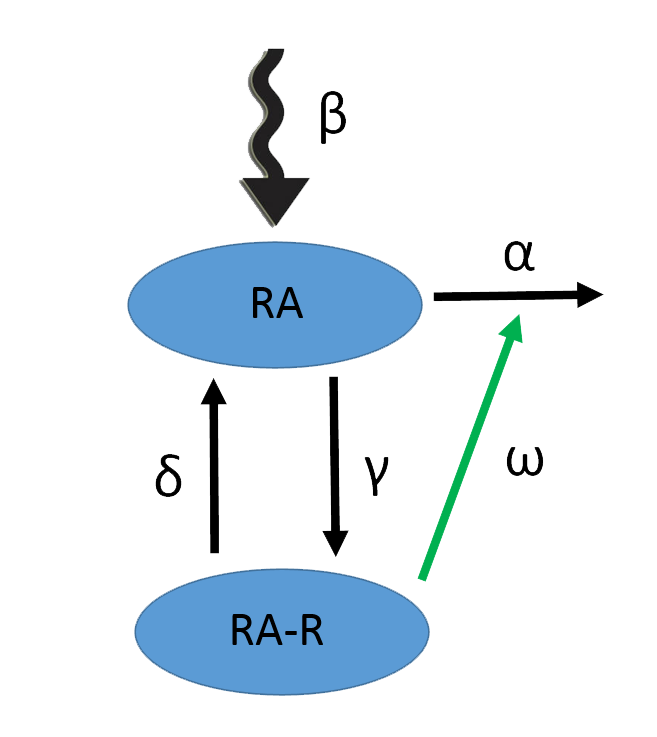
\includegraphics[scale=0.34]{figures/RAPNetwork.PNG}}
\end{tabular}

\footnotesize
\begin{eqnarray*} 
d[RA] & = & [\beta-\left(\frac{\alpha_{0}[Cyp]_{max}[RA-R]}{\omega_{0}/[Crabp]+\omega_{1}+[RA-R]}+\gamma_{0}[Crabp]+\gamma_{b}+\eta\right)[RA] \\
& & + \delta[RA-R] ]dt+\sigma dW_{t}\\
d[RA-R] & = & \left((|\gamma_{0}[Crabp]+\gamma_{b})[RA]-\delta[RA-R]\right)dt\\
d[Crabp] & = & 0
\end{eqnarray*}



}

\boxit{below of = box3, col=1, name=box4}{The Fluctuation-Dissipation Theorem}{
	We can write a system of stochastic differential equations
as
\[
dX=\mu(X,t)dt+\Gamma(X,t)dW_{t},
\]
Take the Jacobian of the deterministic system around a steady state $X_{ss}$ to get
\[
dX=J_{\mu}(X_{ss},t)dt+\Gamma(X_{ss},t)dW_{t}.
\]
The Fluctuation-Dissipation Theorem states that the variance-covariance matrix, $\Sigma$, can be found using the formula
\[
J_{\mu}(X_{ss},t)\Sigma(X_{ss},t)+\Sigma(X_{ss},t)J_{\mu}^{T}(X_{ss},t)=-\Gamma^{2}(X_{ss},t).
\]
 
}


\boxit{below of = box4, col = 1, name=solution}{Solution}{
	WLOG, $\delta=1$. Define the function:
\[
\sigma_{[RA]}^{2}(\alpha,\beta,\omega,\eta,\delta,\gamma)\approx\sigma^{2}f(\alpha,\beta,\eta,\omega,\gamma)
\]


Since during Crabp2a knockdown $\alpha\gg1$, $\frac{\partial f}{\partial\omega}\approx0$.

Let the total change from a knockdown be defined as
\[
\Delta_{\zeta}f=\vert\lim_{\zeta\rightarrow\infty}f-\lim_{\zeta\rightarrow0}f\vert.
\]

\[
\Delta_{\alpha}f=\frac{2(1+\eta)}{4\eta(\gamma+1+\eta)}=\frac{1}{2\eta}\frac{1+\eta}{\gamma+1+\eta}\approx0
\]
 if $\gamma\gg\frac{1}{\eta}$ during Cyp knockdown. And since $\alpha\gg1$
during Crab knockdown,

\[
\Delta_{\gamma}f\approx\frac{1}{2\eta}
\]
 which is large if $\eta\ll1$.

}

\boxit{at top,col = 2, name=conclusions}{Conclusions}{
	\begin{tabular}{c c}
\hspace{-15pt}
{\parbox{.5\textwidth}{
\begin{itemize}
\item We assume the basal rate of RA degradation is "small but not insignificant" and the binding rate of RA to RA-R is large.
\item Knockdown of Cyp26a1:
\begin{itemize}
\item The mean increases.
\item The variance is unchanged.
\end{itemize}
\item Knockdown of Crabp2a:
\begin{itemize}
\item The mean is unchanged.
\item The variance increases.
\end{itemize}
\end{itemize}}}
&
\raisebox{-.45\totalheight}{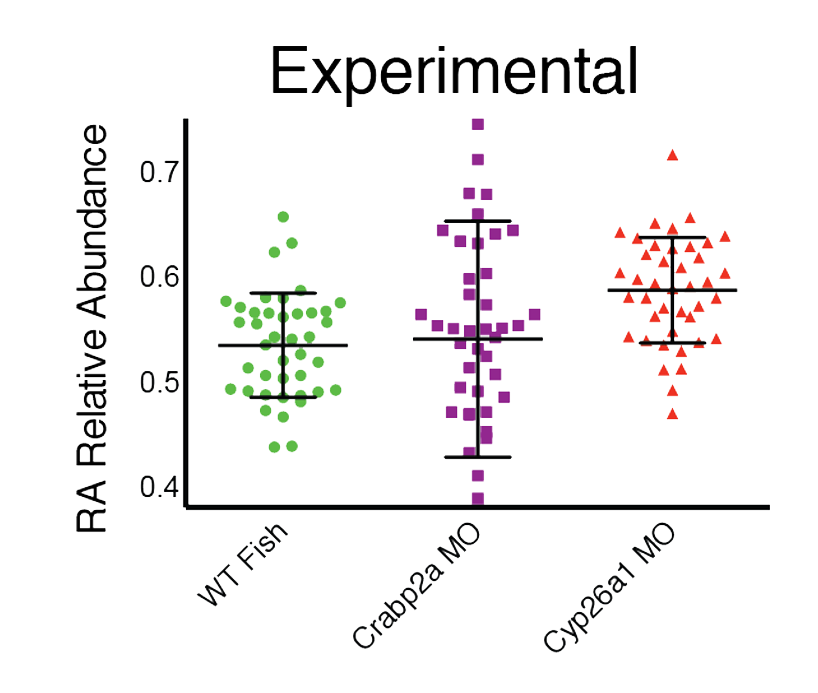
\includegraphics[scale=0.27]{figures/crabNcypKnockdown}}
\end{tabular}
	\vspace{4pt}
}

\boxit{below of = conclusions,col = 2, name=future}{Future Directions}{
	\begin{itemize}
\item Incorporate additional effects into the model.
\begin{itemize}
\item RA upregulates Crabp2a.
\item There limited amounts of receptors.
\end{itemize}
\item Investigate the effects of Cyp26b1 and Crabp2b proteins.
\item Examine the regulatory effects due to transcriptional delays mathematically.
\item Determine the color of the noise.
\begin{itemize}
\item Mathematically determine the approximate color of the noise.
\item Investigate whether the color of the noise holds any information such as temporal delays.
\item Develop an experimental method in order to accurately measure noise frequencies.
\end{itemize}
\item Examine the spatial properties of the noise.
\begin{itemize}
\item Extend the model to a spatial dimension.
\item Perturb the spatial noise using mosaic spatial misexpression experiments.
\end{itemize}
\item Look into the transition events in hindbrain development.
\begin{itemize}
\item Examine both mathematically and experimentally critical transition behaviors through the autocorrelation lags, variance changes, "flickering", spatial coherence.
\end{itemize}
\end{itemize}
	\vspace{4pt}
}

\boxit{col=2, below of= future, name = refs}{Acknowledgments}{
	\vspace{3pt}
	This investigation was supported by the National Institute of Biomedical Imaging and Bioengineering, National Research Service Award EB009418 from the University of California, Irvine, Center for Complex Biological Systems. I would like to thank Professor Qing Nie for his mentorship and Dr. Julian Sosnik for his time and effort.
	\vspace{6.3pt}
}


\end{document}
